\section{Control}

To simplify the dynamic control of the UVMS the author proposes a fuzzy aproach to deal with the complexity of the vehichle-manipulator coupling effect. This can be implemented in a fuzzy kinematic control law giving reference trajectories to the dynamic control laws for the vehichle and manipulator.

\subsection{Force control}

The application of the force control is to do a hot stab operation. This is done much in the same way as a peg-in-hole assembly, which is widely studied in robotic litterature. We will attach a frame to the point the hot stab is done, which serves as a reference frame for the end effector of the manipulator. In spatial impedance control (citation needed) one frame is attached to the robot end effector, another frame is attached as a reference frame to the control system, and a third is attached to the environment, i.e. the hot stab insertion point system, and a third is attached to the environment, i.e. the hot stab insertion point.   

\subsection{Force Control 2}
\begin{figure}[h!]
	\centering
	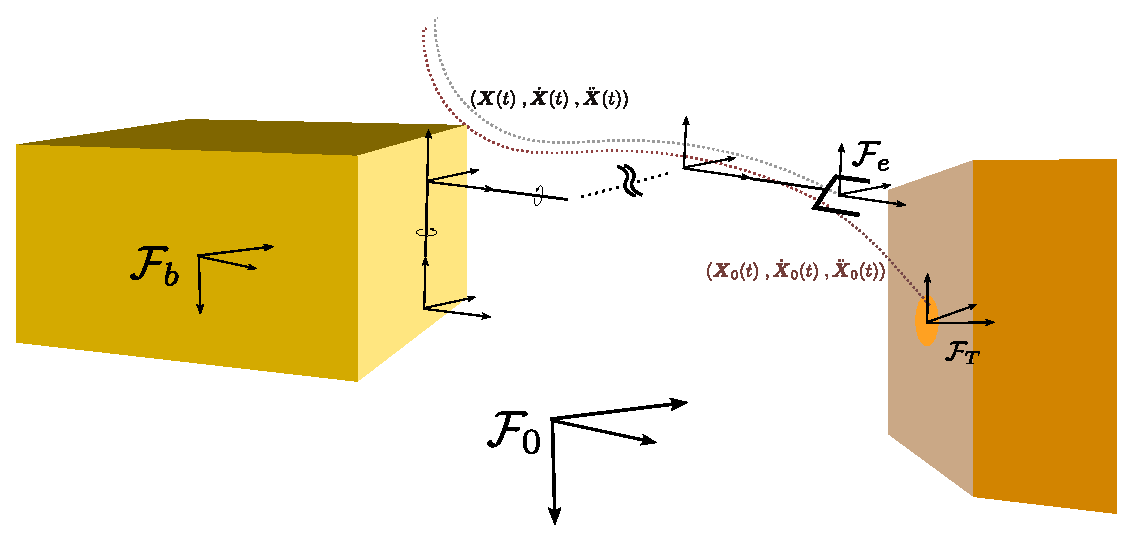
\includegraphics[scale=0.7]{./figures/uvms_kinematics_force.eps}
	\caption{Frames of the UVMS with the inertial and task frame}
	\label{fig:uvms_force}
\end{figure}
The force control is analyzed in the task space, as observed by the end effector, and we can define the forces acting upon the manipulator due to contact with the environment 
\begin{align}
	\bs F_e^e&=\begin{bmatrix} f_x & f_y & f_z & m_x & m_y & m_z \end{bmatrix}
	\label{eq:force_force}
\end{align}
$\bs F_e^e$ is therefor the same as $\bs F$ defined in \eqref{eq:jacobian_force} and can therefor be mapped into the joint the general forces $\taub$ by the transpose jacobian
\begin{align}
	\taub&=(\jb{ge}{B})^T\bs F_e^e
	\label{eq:jacobian-force2}
\end{align}
Let the translational part of the trajectory of the end effector be defined as

\begin{align}
	\bs X(t) \; , \; \dot{\bs X}(t)\; , \; \ddot{\bs X}(t)	
	\label{eq:ee_traj}
\end{align}
Which gives the position, velocity and acceleration of the end effector relative to the task frame \frame T, illustrated in Fig. \ref{fig:uvms_force}. Further we will define a nominal trajectory which represents the planned trajectory, given by a path plan algorithm and/or an operator

\begin{align}
	\bs X_0(t) \; , \; \dot{\bs X}_0(t)\; , \; \ddot{\bs X}_0(t)	
	\label{eq:nominal_force}
\end{align}
We can then model the force due to interaction, when the end effector is in contact with the environment, \cite{impedance_stability}

\begin{align}
	\bs F&=\bs K(\bs X - \bs X_0) + \bs B(\dot{\bs X} - \dot{\bs X}_0) + \bs J(\ddot{\bs X} - \ddot{\bs{X}}_0)
	\label{eq:ee_impedance1}
\end{align}
The nominal path can then be interpreted as the no contact path. The constants $\bs K$, $\bs B$ and $\bs J$ can then be regarded as the desired stiffness, damping and inertia of the end effector in contact with the environment. The impedance defined in \eqref{eq:nominal_force} can then be obtained either by direct force control, or it can be used to adjust the path of the endeffector, relying on an inner position control loop. In this paper the latter will be discussed. \cite{impedance_stability} proposes an adjustment vector $\bs X_a$ which is a result of filtering $\bs F$ through a second order low pass filter

\begin{align}
	\bs X_a(s)&= \frac{1}{(\bs K+\bs Bs+ \bs Js^2)}\bs F(s)
	\label{eq:x_adjusted}
\end{align}
$\bs X_a$ can then be seen as a perturbation from the nominal path due to the desired impedance, as defined in \eqref{eq:ee_impedance1}. We will, for the sake of simplicity only consider diagonal $\bs K$, $\bs B$ and $\bs J$ matrices, so that the forces are decoupled. The commanded trajectory that is used as the input for the motion control loop can then be written as
\begin{align}
	\bs X_c&= \bs X_0 + \bs X_a
	\label{eq:controlled_traj}
\end{align}




